\documentclass[a4paper]{article}

\usepackage{amsmath}
\usepackage{physics}
\usepackage{hyperref}
\usepackage[all]{hypcap} % Make a hyperlink navigate to the top of the figure
\usepackage{graphicx}
\graphicspath{ {./images/} }
\usepackage[a4paper,left=3cm,right=3cm,top=2.5cm,bottom=2.5cm]{geometry}

\title{Quantum Phase Estimation}
\author{Tzu Hsuan Chang}

\begin{document}
\maketitle

\section{Introduction}
\label{sec:Intro}
Quantum phase estimation (QPE) is used to find the eigenvalues of a unitary matrix. Suppose we want to find the eigenvalues $e^{2 \pi i \theta_i}$ corresponding to the eigenvector $\ket {u_i}$ of an unitary operator $\hat{U}$ such that
$\hat{U} \ket{u_i}  = e^{2 \pi i \theta_i} \ket{u_i}$. The QPE have the following operation,
    \begin{equation} \label{eq:eq1}
    \setlength{\jot}{10pt}
        \ket{0} \ket{u_i}   \longrightarrow   \ket{\tilde \theta_i} \ket{u_i},
    \end{equation}
where $\tilde \theta_i$ is an estimate for $\theta_i$.

As shown on figure~\ref{fig:qpe}, the QPE circuit write the phase of $\hat U$ to n ancillary qubits $\ket{0}^{\otimes n}$ in the Fourier basis and using inverse QFT to transform them back to the computational basis. The following is the mathematical details.

\subsection*{Mathematical details}
\label {subsec:qpe}

As shown in figure~\ref{fig:qpe}, assuming $\psi$ is the eigenvector of the unitary operator $\hat U$ with eigenvalue $e^{2 \pi i \theta}$. Initially, we have
    \begin{equation} \label{eq:eq2}
    \setlength{\jot}{10pt}
        \ket{\psi_0}   =   \ket{0}^{\otimes n} \psi.
    \end{equation}
After applying n-bit Hadamard gates on the ancillary qubits,
    \begin{equation} \label{eq:eq3}
    \setlength{\jot}{10pt}
        \ket{\psi_1}   =   \frac{1}{2^{n/2}} (\ket{0} + \ket{1})^{\otimes n} \psi.
    \end{equation}
Now we apply controlled unitary operator $C-U$. Since $\ket{\psi}$ is the eigenvector fo $\hat{U}$, we have,
    \begin{equation} \label{eq:eq4}
    \setlength{\jot}{10pt}
        \hat{U}^{2^j} \ket \psi   =   \hat{U}^{2^j - 1} \ e^{2 \pi i \theta} \ket{\psi}   =   e^{2 \pi i 2^j \theta} \ket{\psi}.
    \end{equation}
By apply all the n controlled operations,
    \begin{equation} \label{eq:eq5}
    \setlength{\jot}{10pt}
    \begin{aligned}
        \ket{\psi_2}   &=   \frac{1}{2^{\frac{n}{2}}}   \big(\ket{0} + e^{2 \pi i \theta 2^{n-1}} \ket{1} \big)
        \otimes \dotso 
        \otimes \big(\ket{0} + e^{2 \pi i \theta 2^{1}} \ket{1} \big)
        \otimes \big(\ket{0} + e^{2 \pi i \theta 2^{0}} \ket{1} \big)
        \otimes \ket{\psi} \\
        &=   \frac{1}{2^{\frac{n}{2}}}   \sum_{k=0}^{2^n - 1}   e^{2 \pi i \theta k} \ket{k}   \otimes \ket{\psi},
    \end{aligned}
    \end{equation}
where $k$ is the integer representation of n ancillary qubits.
Finally, we are going to apply inverse QFT to get the phase estimate of $\theta$. Note that QFT is the following operation,
    \begin{equation} \label{eq:eq6}
    \setlength{\jot}{10pt}
        QFT \ket{j}   =   \frac{1}{2^{\frac{n}{2}}}   { \big( \ket{0} + e^{2 \pi i \frac{j}{2}} \ket{1} \big)
        \otimes \big( \ket{0} + e^{2 \pi i \frac{j}{2^2}} \ket{1} \big)
        \otimes \dotso 
        \otimes \big( \ket{0} + e^{2 \pi i \frac{j}{2^n}} \ket{1} \big) }.
    \end{equation}
With $j$ replaced by $2^n \theta$, we have the following states after applying inverse QFT to the ancillary qubits,
    \begin{equation} \label{eq:eq7}
    \setlength{\jot}{10pt}
        \ket{\psi_3}   =   QFT^\dagger_n   \ket{\psi_2}
        = QFT^\dagger_n   \frac{1}{2^{\frac{n}{2}}}   \sum_{k=0}^{2^n - 1}   e^{2 \pi i \theta k} \ket{k}   \otimes \ket{\psi}
        = \frac{1}{2^{\frac{n}{2}}}    \sum_{j=0}^{2^n - 1}   \sum_{k=0}^{2^n - 1}   e^{ -\frac{2 \pi i k}{2^n} (j - 2^n \theta)} \ket{j}   \otimes \ket{\psi}.
    \end{equation}
    We can find that there is a peak near $j = 2^n \theta$. Therefore, by measuring ancillary qubits in the computational basis, we would get the phase with high probability,
    \begin{equation} \label{eq:eq8}
        \ket{\psi_4}   =   \ket{2^n \theta} \otimes \ket{\psi}.
    \end{equation}

    \begin{figure}
        \centering
            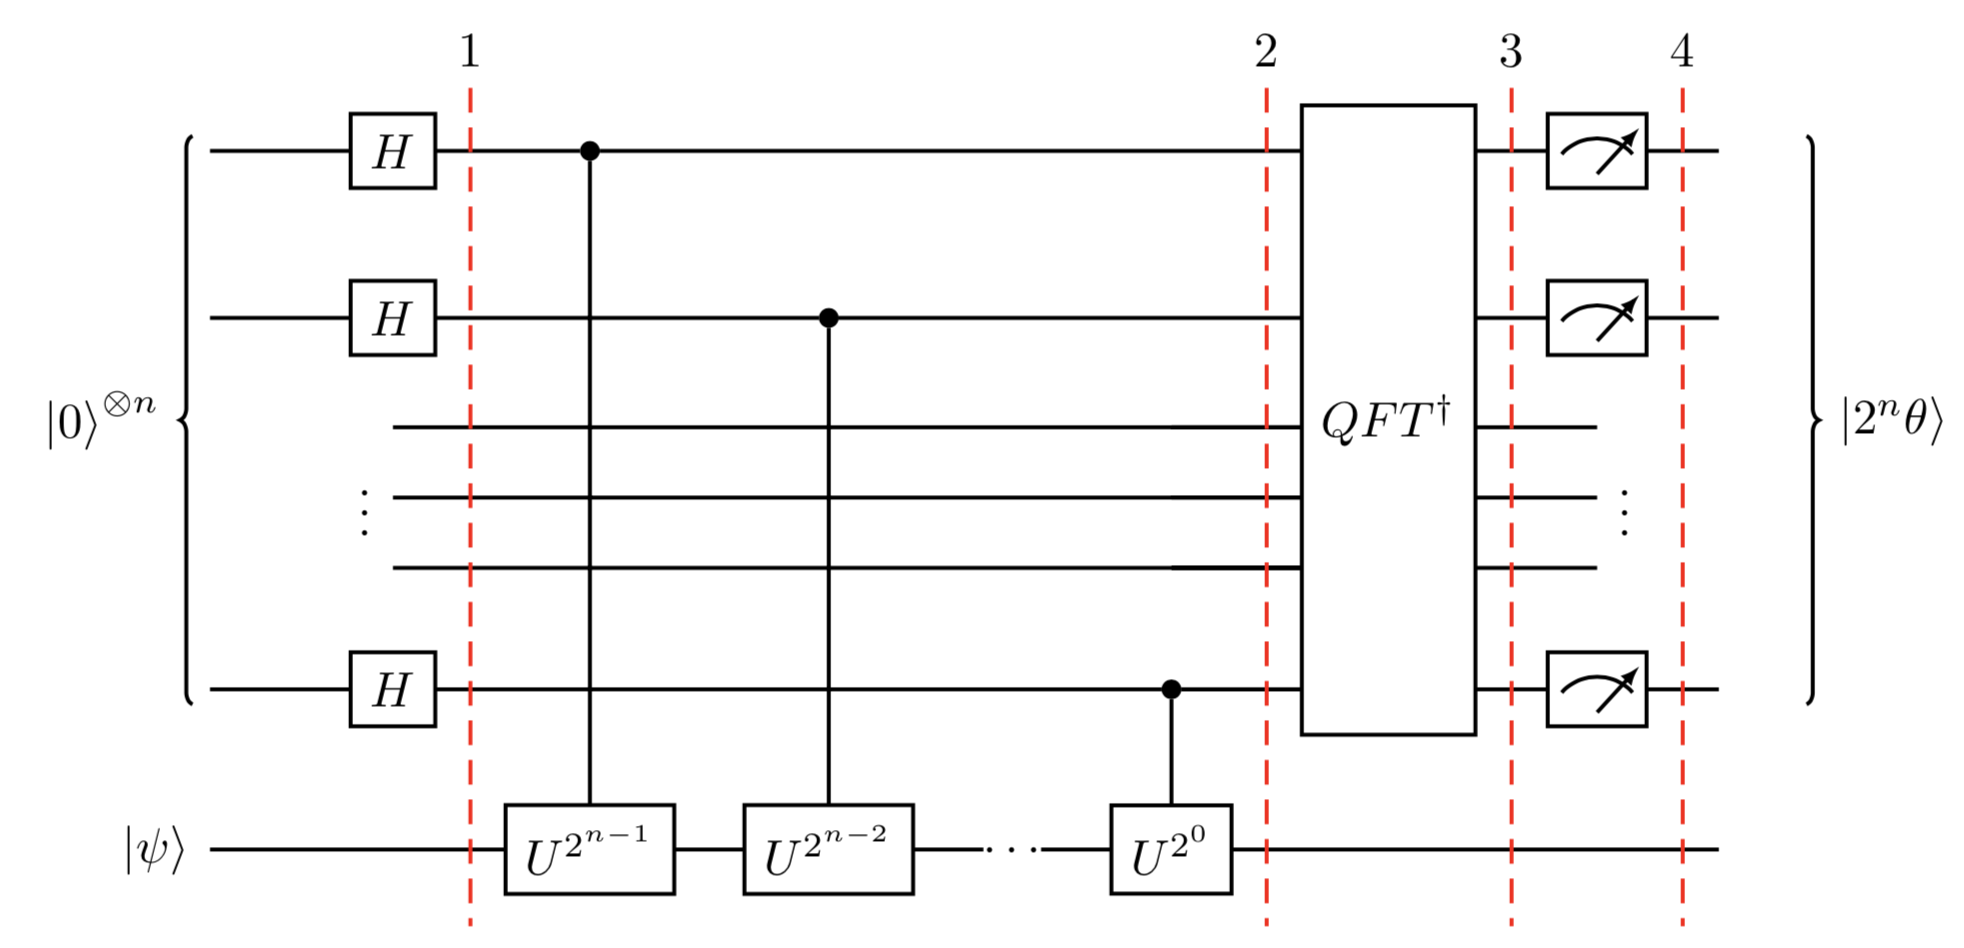
\includegraphics [width=\textwidth, height=\textheight, keepaspectratio] {qpe_tex_qz.png}
        \caption{Quantum phase estimation circuit.\cite{Qiskit-Textbook}}
        \label{fig:qpe}
    \end{figure}


\bibliographystyle{abbrv}
\bibliography{references}

\end{document}